\chapter{Electric characterization}
\label{ch:electric} 
The development of electric components used to produce the Plasma Coagulation Controller is highly influenced by the need of flexibility in settings and mobility for wound treatment. To produce plasma as DBD, in air with Helium or Argon as ignition gasses, it is necessary to produce high voltage, to permit easy medical application the design of the head must be compact with particular attention to electric safety measuraments.
The scheme outputs a voltage pulse with an amplitude up to $\SI{10}{\kilo\volt}$ and frequencies up to $\SI{50}{\kilo\hertz}$.

A rappresentation of power and signal line is in figure \ref{fig:electricline}. The circuit is divided mainly in two parts %as described in chapter \ref{ch:source}
: the controller, with alimentation and settings controls, and the head, where the discharge happens and plasma is emitted.
\begin{figure}
 \centering
 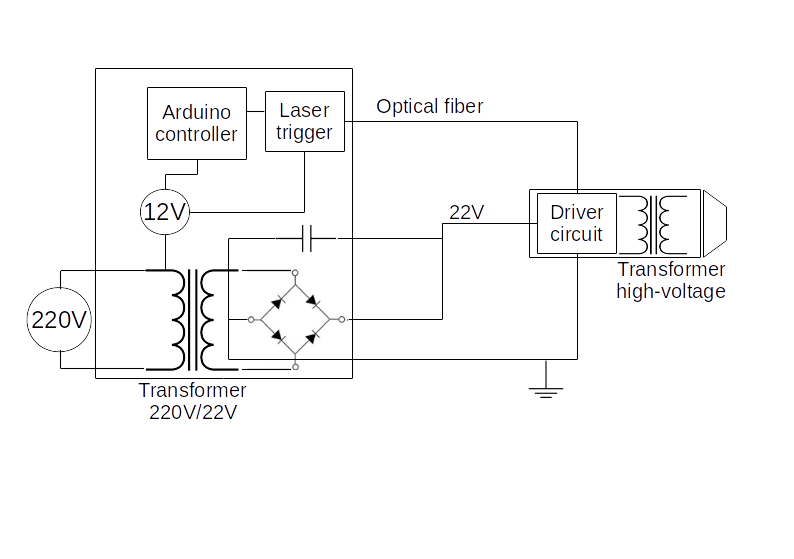
\includegraphics[width=0.8\textwidth]{Images/Linea_elettrica.png}
 \caption{Scheme of the general electric line to produce high voltage, the controller on the left and the head on the left.}
 \label{fig:electricline}
\end{figure}

The line divides in:
\begin{itemize}
 \item \bf{Alimentation} : the $\SI{220}{\volt}$ DC power line goes in a transformer that gives a $\SI{22}{\volt}$ tension to the head, passing through a diode bridge. This tension aliments the driver circuit on the head.
 \item \bf{Arduino and trigger} : the power line is reduced to $\SI{12}{\volt}$ necessaries to aliment an Arduino controller and a laser. From an analogical output of the Arduino a PWM wave goes to the laser trigger, it transmit information on the wave frequency and duration with an optical fiber that ends with a photodiode installed on the driver circuit. Wave frequency is setted by the Arduino, wave duration is setted giving the opengin time of the MOSFET installed on the driver circuit. With this setup the High-Voltage line is entirely decopuled from the controller, in this way there are not serious problems of signal reflection on the power line or the Arduino.
 \item \bf{Head} : the Driver Circuit receives a power line of $\SI{22}{\volt}$ and an optical trigger that defines frequency and duration of the voltage pulse. When the trigger gives the start signal the transformer on the head receives on primary circuit a voltage of hundreds $\si{\volt}$ and outputs from secondary circuit a voltage of thousends $\si{\volt}$. Connected to the ouput there is an electrode inside a capillary tube.
\end{itemize}


A simulation of the different signals, obteined with a simplified scheme with Spice, is in figure \ref{fig:signals}. As in the figure...

The characterization of the electric scheme is made measuring output tension and current with different settings for the pulse.


\begin{comment}
La sorgente di plasma funziona tramite l'applicazione di un'alta differenza di potenziale tra gli elettrodi separati da materiale dielettrico, come descritti nel capitolo \ref{ch:sorgente}. La tensione in ingresso nel circuito  della testa della sorgente vengono amplificati fino a tensioni di alcuni \si{\kilo\volt}. Dall'arduino di controllo è possibile regolare il tempo di apertura del circuito in un range di [$2$-$20$] \si{\micro\second} e la frequenza di lavoro in un range di [$2$-$60$] \si{\kilo\hertz}. I parametri importanti per caratterizzare il funzionamento della sorgente saranno quindi tensione e corrente all'uscita del circuito secondario del trasformatore, al variare dei parametri di funzionamento. Utilizzando una lastra metallica posta a potenziale, è possibile misurare la corrente in un dato range temporale. È inoltre possibile stimare la corrente efficace che attraversa il bersaglio, importante nel valutare gli effetti dell'applicazione del plasma.

\section{Setup delle misure di tensione e corrente}
Si vogliono effettuare misure di tensione della sorgente sia senza immissione di elio, senza formazione della plume di plasma, sia nelle condizioni di funzionamento tipiche, con flusso di elio di $\SI{2}{\liter/\minute}$.
Le tensioni vengono misurate tramite una sonda \emph{...} con attenuazione $\times1000$, le correnti tramite una sonda \emph{Tektronix CT2} che per una corrente di \SI{1}{\milli\ampere} restituisce un segnale di \SI{1}{\milli\volt}. I dati vengono letti su un oscilloscopio \emph{Yokogawa DL9040}, che permette il salvataggio dell'intera forma d'onda misurata nei diversi canali. 
Viene effettuata la caratterizzazione elettrica di entrambi i prototipi di sorgente, per i quali il circuito utilizzato è lo stesso, quindi non si aspettano variazioni significative.

\subsection{Misure senza elio}
La sonda ad alta tensione viene collegata all'uscita del circuito secondario, mentre una sonda con attenuazione $\times10$ viene utilizzata per controllare il segnale in ingresso.
La sorgente viene azionata variando la frequenza ($f$) e duty cycle ($\Delta t$). Scelta la frequenza di lavoro, viene variata la duty cycle in un range utile, considerando il tempo necessario al terminare delle oscillazioni del segnale prima dell'arrivo di una nuova onda quadra (per frequenze maggiori si potrà arrivare a duty cycle minori).
Si ottengono curve come in figura \ref{fig:tensione_es}. La risoluzione della misura viene variata in modo da avere l'errore di misura minore possibile.

\begin{figure}
\centering
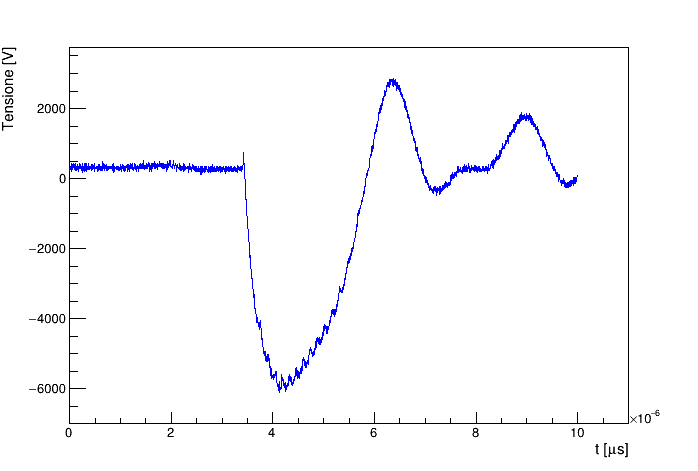
\includegraphics[width=.7\textwidth]{Immagini/tensione_es_2.png}
\caption{Esempio di misura di tensione, $f = \SI{5}{\kilo\hertz}$ e $\Delta t = \SI{16}{\micro\second}$, prototipo 1.}
\label{fig:tensione_es}
\end{figure}

\subsection{Misure con elio}
Per caratterizzare il funzionamento della sorgente nelle possibili condizioni di trattamento, vengono misurate contemporaneamente, su due diversi canali dell'oscilloscopio, tensione alla quale si trova l'elettrodo e corrente che fluisce nel plasma. Per la misura di corrente viene fatto impattare il plasma su una piastra di rame  di dimensioni \SI{2}{\centi\metre} $\times$ \SI{2}{\centi\metre} $\times$ \SI{0.5}{\centi\metre}, ad una distanza di \SI{1}{\centi\metre} dall'elettrodo della sorgente, collegata alla sonda di corrente.
Nuovamente vengono effettuate misure al variare di frequenza ($f$) e duty cycle ($\Delta t$), con le stesse modalità delle misure di tensione.
Tutte le misure sono effettuate con flusso di gas He pari a $\SI{2}{\litre/\minute}$.
Si ottengono curve come in figura \ref{fig:corrente_es}.

\begin{figure}
\centering
 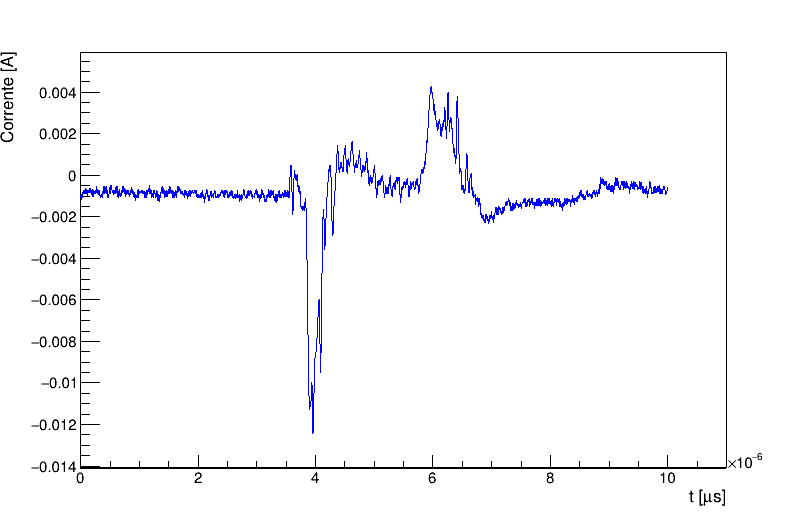
\includegraphics[width=.7\textwidth]{Immagini/corrente_es.png}
\caption{Esempio di misure di corrente per $f = \SI{5}{\kilo\hertz}$ e $\Delta t = \SI{24}{\micro\second}$, prototipo 1.}
\label{fig:corrente_es}
\end{figure}


\section{Presentazione misure ed analisi}
Sia per le misure di tensione che per le misure di corrente si trova un picco negativo come presentato nelle Figure \ref{fig:tensione_es} e \ref{fig:corrente_es}. Il picco di tensione ha valori tipici tra i $\num{3}$ e i $\SI{10}{\kilo\volt}$ in assenza o in presenza di gas, mentre quello di corrente tra i $\num{2}$ e i $\SI{12}{\milli\ampere}$.
L'analisi dei dati prevede la ricerca del massimo della tensione e della corrente nelle diverse configurazioni.

\subsection{Tensione di picco senza elio}
L'andamento medio delle misure presenta un picco negativo pronunciato, compatibile con i tempi di apertura del circuito. Dato un set, il valore di picco viene cercato calcolando la trasformata di Fourier del segnale (tramite le routine fftw3 delle librerie ROOT), tagliando le oscillazioni ad alta frequenza e ricostruendone una media. Nel segnale medio così ricostruito il valore del minimo viene trovato interpolando con una funzione di Landau attorno il minimo, in modo da riprodurre l'asimmetria del picco.
A queste misure viene aggiunto l'errore dovuto al taglio delle alte frequenze, preso come una media del valore assoluto dell'oscillazione del segnale tagliato. Viene inoltre aggiunto l'errore caratteristico dello strumento di misura, trascurabile rispetto l'errore dovuto alle oscillazioni veloci.
In figura \ref{fig:landau} un esempio del fit.

\begin{figure}
\centering
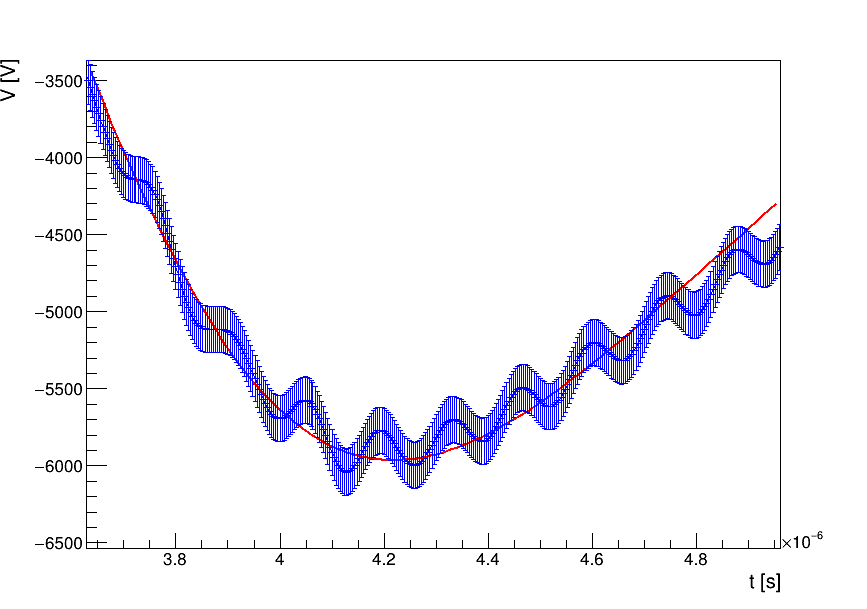
\includegraphics[width=.6\textwidth]{Immagini/esfiterr.png}
\caption{Esempio di fit del picco di tensione, $f = \SI{5}{\kilo\hertz}$ e $\Delta t = \SI{16}{\micro\second}$}
\label{fig:landau}
\end{figure}


Le tensioni del picco così calcolate, al variare della duty cycle per le diverse frequenze, sono presentate in figura \ref{fig:tensioni}.
Per tutte le frequenze di lavoro tra i $\SI{4}{\micro\second}$ e i $\SI{16}{\micro\second}$ risulta un andamento lineare, con tensione variabile tra i $\SI{2}{\kilo\volt}$ e i $\SI{9}{\kilo\volt}$. Aumentando ancora il tempo di apertura del circuito la tensione arriva a valori più elevati, fino un massimo di circa $\SI{10}{\kilo\volt}$, ma viene perso l'andamento lineare.


 \begin{figure}
\centering
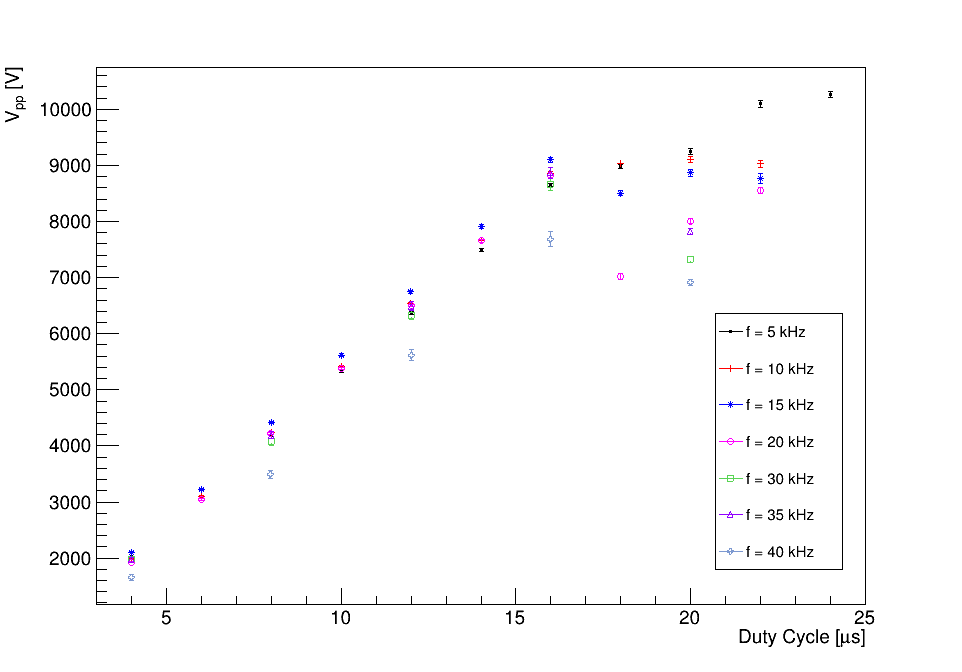
\includegraphics[width=.6\textwidth]{Immagini/nogas.png}
\caption{Tensioni al variare del tempo di apertura del circuito e per diverse frequenze.}
\label{fig:tensioni}
\end{figure}


Le misure non sembrano presentare un andamento in funzione della frequenza, per verificarlo vengono calcolati i coefficenti dell'interpolazione lineare per le varie frequenze, presentati in figura \ref{fig:fitlin}.
Viene confermata l'assenza di un andamento specifico al variare della frequenza.

\begin{figure}
\centering
\subfloat[][Pendenza delle rette.]
  {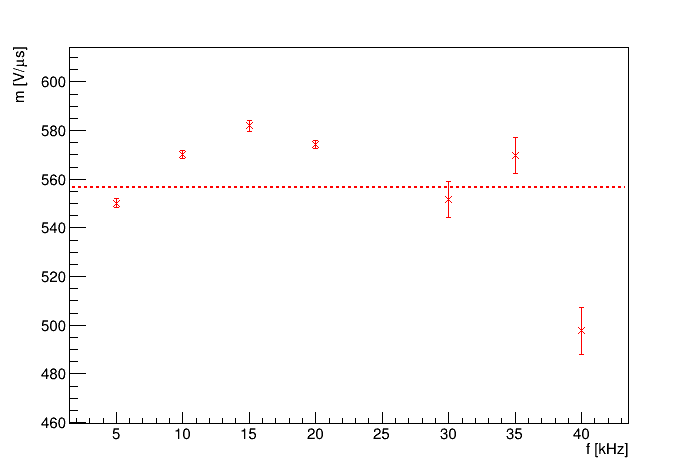
\includegraphics[width=.48\textwidth]{Immagini/m_freq_nogas.png}}
\subfloat[][Intercetta delle rette.]
  {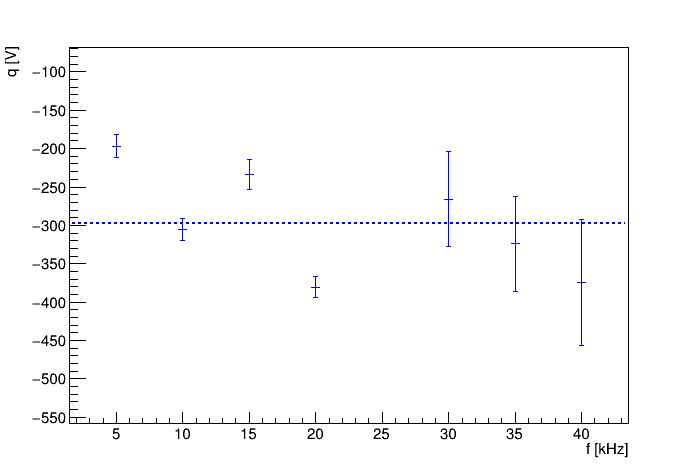
\includegraphics[width=.48\textwidth]{Immagini/q_freq_nogas.png}}
\caption{Parametri dell'interpolazione lineare dei set di misure senza immissione di gas(nel range $\Delta t$ stabilito), al variare della frequenza.}
\label{fig:fitlin}
\end{figure}


\subsection{Tensione e corrente con elio}
Le misure di tensione presentano l'andamento trovato precedentemente, mentre le misure di corrente presentano un primo picco negativo seguito da un picco più basso di segno opposto, positivo. L'analisi proposta è uguale a quella pensata per i set di misure precedenti: vengono tagliate le oscillazioni ad alta frequenza, ricostruito il segnale (aggiungendo l'errore dovuto al taglio delle alte frequenze e agli strumenti di misura) e il valore del minimo viene trovato interpolando con una funzione di Landau. Da questo fit vengono calcolati valori e posizione del picco di tensione, del picco negativo di corrente e del picco positivo di corrente.
In figura \ref{fig:landau} un esempio del fit.

\begin{figure}
\centering
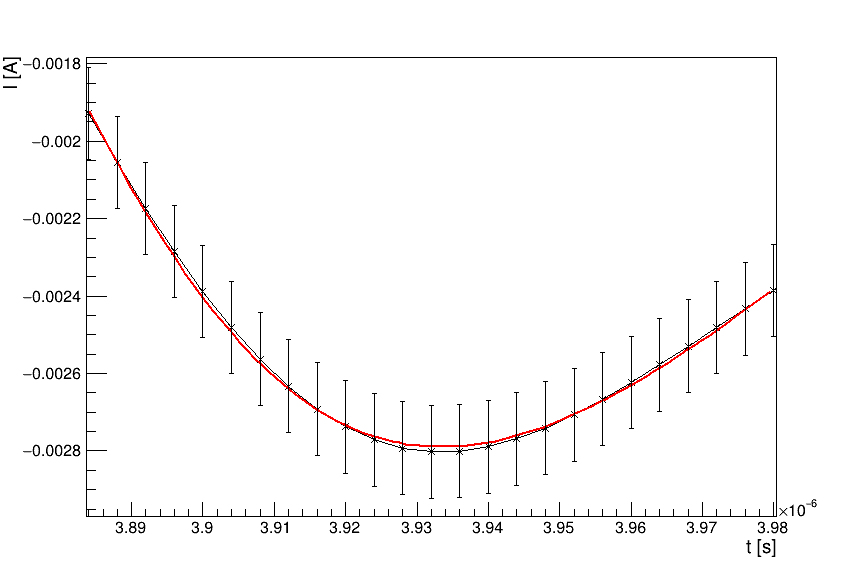
\includegraphics[width=.6\textwidth]{Immagini/es_fit_landau.png}
\caption{Esempio di fit del picco di corrente, $f = \SI{5}{\kilo\hertz}$ e $\Delta t = \SI{24}{\micro\second}$}
\label{fig:landau}
\end{figure}

Le tensioni del picco così calcolate, al variare della duty cycle per le diverse frequenze, sono presentate in figura \ref{fig:picchi}.
Nuovamente troviamo un andamento lineare per la tensione tra i $\num{4}$ e i $\SI{16}{\micro\second}$. Anche il picco negativo di corrente presenta questo andamento lineare, mentre per il picco positivo non è possibile identificare un comportamento simile, i valori si disperdono.

\begin{figure}
\centering
\subfloat[][Modulo del picco di tensione.]
  {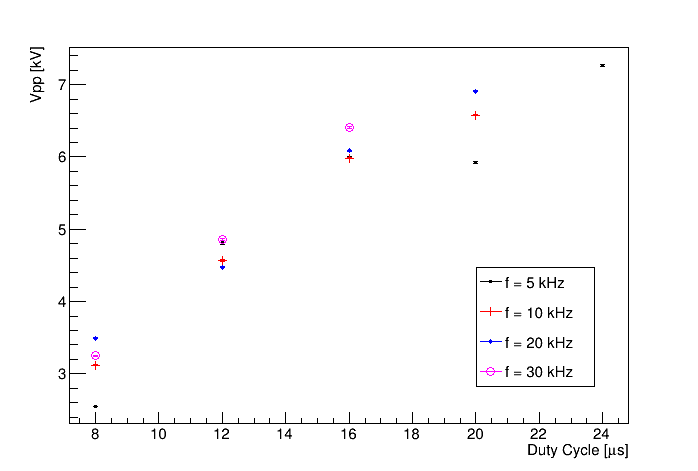
\includegraphics[width=.65\textwidth]{Immagini/vpp_corrente.png}}
\\
\subfloat[][Modulo del picco primario di corrente.]
  {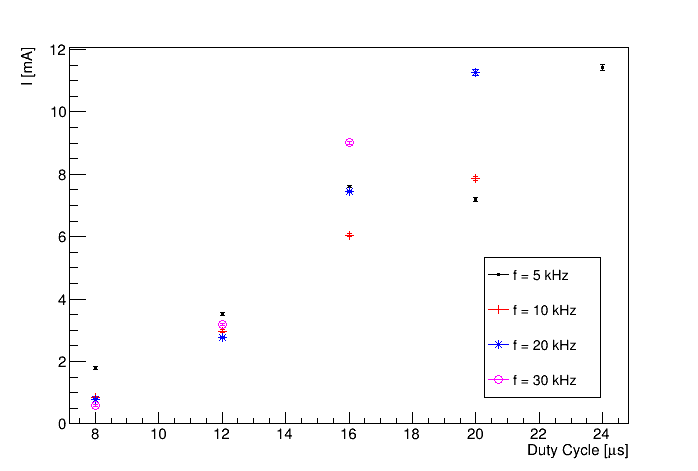
\includegraphics[width=.65\textwidth]{Immagini/I1_corrente.png}}
\\
\subfloat[][Picco secondario di corrente.]
  {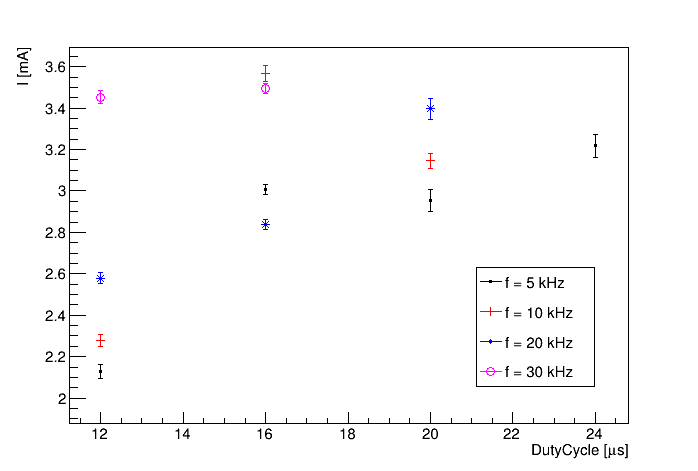
\includegraphics[width=.65\textwidth]{Immagini/I2_corrente.png}}
\caption{Valori dei picchi misurati al variare del tempo di apertura del circuito e per diverse frequenze.}
\label{fig:picchi}
\end{figure}


Nuovamente, per visualizzare in maniera esplicita l'effetto della variazione della frequenza, vengono calcolati i coefficenti dell'interpolazione lineare per le tensioni di picco e per le correnti di picco negativo, presentati in figura \ref{fig:fitlin_cor}. 
Per le tensioni risulta un comportamento identico al precedente, dove i valori si assestano attorno una media lievemente inferiore rispetto le misure in assenza di elio.
Per il valore massimo di corrente viene trovato un aumento in funzione della frequenza di funzionamento della sorgente.

\begin{figure}
\centering
\subfloat[][Pendenze dei picchi di tensione.]
  {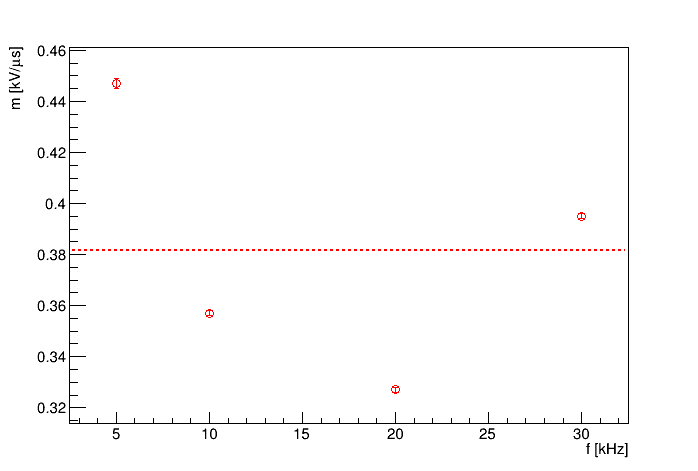
\includegraphics[width=.48\textwidth]{Immagini/mVpp_cor.png}}
\subfloat[][Intercette dei picchi di tensione.]
  {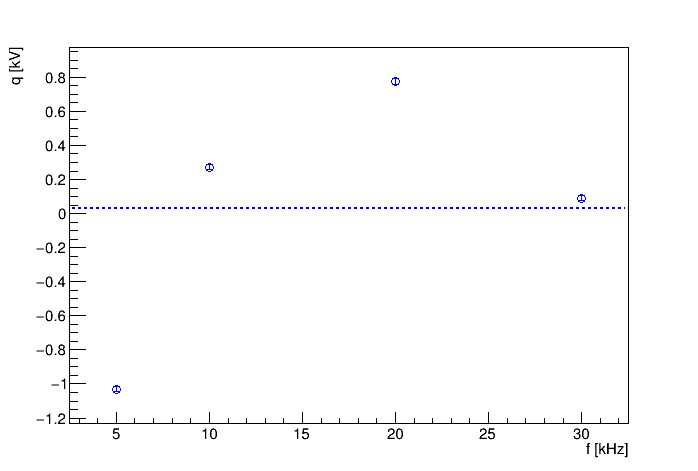
\includegraphics[width=.48\textwidth]{Immagini/qVpp_cor.png}}
\newline
\subfloat[][Pendenze dei picchi di corrente.]
  {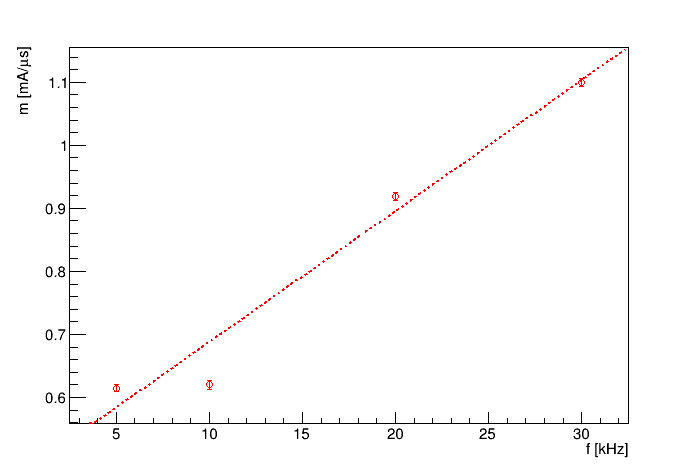
\includegraphics[width=.48\textwidth]{Immagini/mI1_cor.png}}
\subfloat[][Intercette dei picchi di corrente.]
  {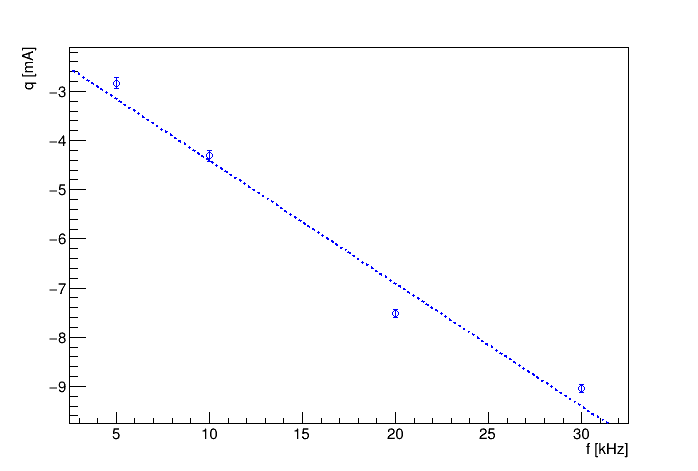
\includegraphics[width=.48\textwidth]{Immagini/qI1_cor.png}}
\caption{Parametri dell'interpolazione lineare dei picchi delle misure di tensione e corrente.}
\label{fig:fitlin_cor}
\end{figure}

\begin{comment}

Data la possibilità di visualizzare contemporaneamente sia la tensione sia la corrente in uscita dal circuito, viene proposta un'analisi delle variazioni temporali tra i diversi picchi. In particolare viene calcolato il tempo tra i due picchi di corrente e tra il picco di tensione e il picco di corrente primario, mostrati in figura \ref{fig:tempi}.
In entrambi i casi non è possibile estrapolare un andamento particolare, indicando che non vi sono differenze significative nei tempi di salita dei picchi al variare del tempo di apertura del circuito e della frequenza.

\begin{figure}
\centering
\subfloat[][Tempo tra i picchi di corrente.]
  {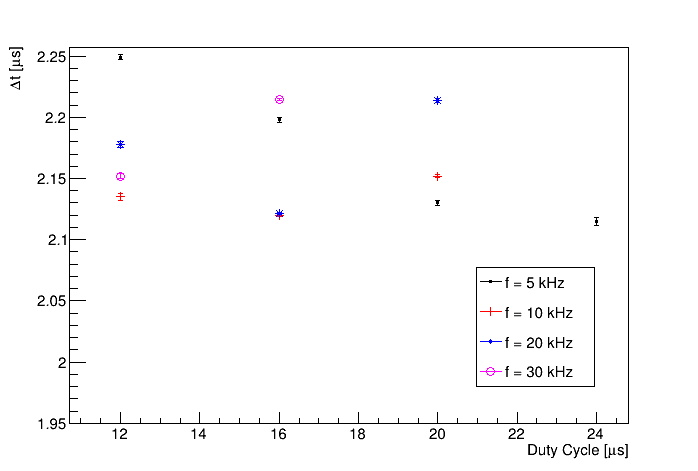
\includegraphics[width=.48\textwidth]{Immagini/ti2ti1.png}}
\subfloat[][Tempo tra picco tensione e primo picco di corrente.]
  {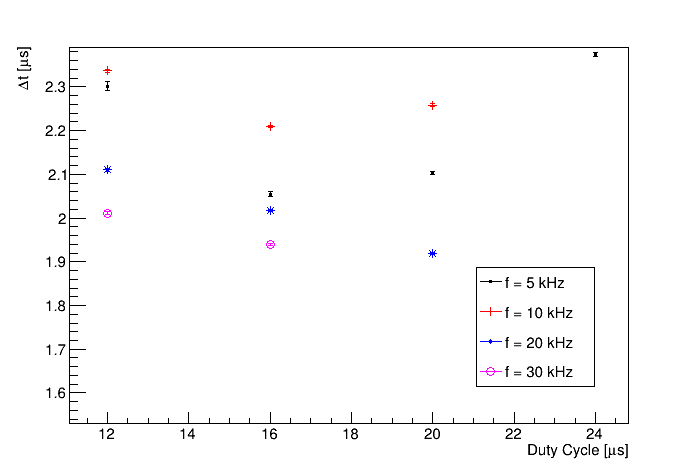
\includegraphics[width=.48\textwidth]{Immagini/ti1tv.png}}
\caption{Misura delle differenze temporali tra i picchi.}
\label{fig:tempi}
\end{figure}

\subsection{Corrente efficace}
Durante l'applicazione del plasma su tessuti vivi bisogna considerare il tempo di reazione effettivo del bersaglio, l'impulso di corrente alle frequenze di lavoro della sorgente presenta un periodo inferiore rispetto questi tempi. Per valutare gli effetti del trattamento viene calcolato il valore della corrente efficace che fluisce sulla piastra bersaglio in un tempo di \SI{1}{\milli\second}, dell'ordine di grandezza dei tempi di risposta da considerare (vedi articolo?), utilizzando la formula in \ref{eq:ieff}.
\begin{equation}
 \centering
 I_{\text{eff}} = \frac{1}{(t_2-t_1)}\sqrt{\int_{t_1}^{t_2} I^2 \,dt}
 \label{eq:ieff}
\end{equation}

In Figura \ref{fig:correff} vengono presentati i valori della corrente efficace in maniera simile a quanto fatto per le misure di corrente precedentemente.
A parità di tempo di apertura del circuito, una maggiore frequenza implica che nel tempo scelto di \SI{1}{\milli\second} vi sarà un numero di periodi maggiore, aumentando la corrente efficace nel circuito. In figura si vede come mediamente la corrente efficace sia più grande a frequenze maggiori, ma assume sempre valori inferiori ai \SI{3}{\milli\ampere}.

\begin{figure}
\centering
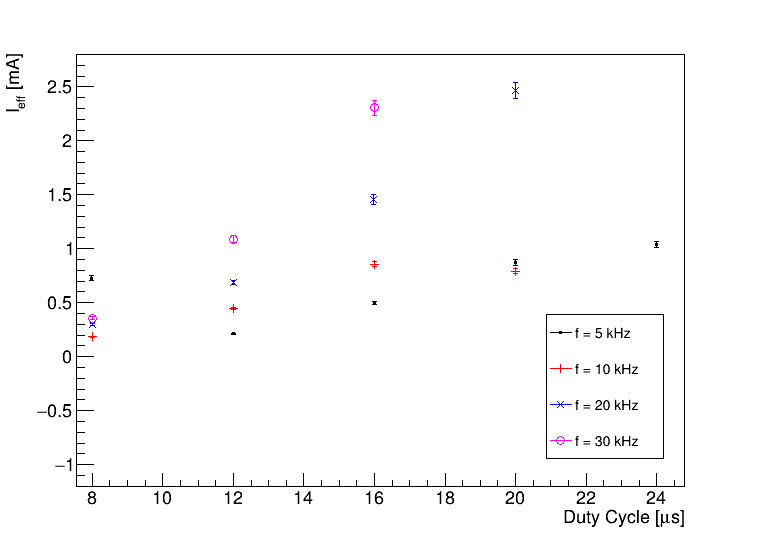
\includegraphics[width=.7\textwidth]{Immagini/ieff.png}
\caption{Corrente efficace calcolata al variare del tempo di apertura del circuito e per diverse frequenze.}
\label{fig:correff}
\end{figure}

\end{comment}
